% Compile from this directory:
%   pdflatex completed_deliverables_report.tex
\documentclass[11pt]{article}
\usepackage[margin=1in]{geometry}
\usepackage{graphicx}
\usepackage{xcolor}
\usepackage{booktabs}
\usepackage{enumitem}
\usepackage{parskip}
% hyperref loads url; set url options first to avoid "Option clash for package url"
\PassOptionsToPackage{hyphens}{url}
\usepackage{hyperref}
\Urlmuskip=0mu plus 1mu

\hypersetup{
  colorlinks=true,
  linkcolor=blue!60!black,
  urlcolor=blue!60!black,
  citecolor=blue!60!black
}

\title{CSE 493S Empirical Methods Assignment\\
\large Progress Report: Finished Deliverables}
\author{ % replace with your name
Aadyant Maity and Rahul Bonthu
}
\date{May 1, 2026}

\begin{document}
\maketitle

\section{Part 0: implementation}

Part~0 is basically the codebase the rest of the assignment builds on. Everything lives under \path{deliverables/part_0/}: the usual scripts (\path{train.py}, \path{model.py}, \path{inference.py}, \path{tokenizer_utils.py}, \path{arith_data.py}) plus \path{part_0_1_contract.py} for the autograder-facing API.

We sanity-check with the quick configs from the README, for example:
\begin{verbatim}
python train.py --config configs/sanity_quick.yaml
python train.py --config configs/sanity_suffix_quick.yaml
\end{verbatim}
(run from the \texttt{EmpiricalHW/} root, or point paths appropriately). Nothing fancy to report here besides ``it trains and the contract loads checkpoints''---the interesting experiments start in Part~1.

\section{Section 1.1: modular arithmetic datasets}

For \S1.1 we generated text files of equations \texttt{a op b = c} with arithmetic mod $p$. Addition and subtraction iterate all pairs $(a,b)$ with $0 \le a,b < p$. Division skips $b=0$ and uses $b \in \{1,\ldots,p-1\}$, so division sets are a bit smaller than add/sub for the same~$p$.

We shuffled once with seed~$0$, then split each file \textbf{80\% / 10\% / 10\%} train, validation, and test in that order. Every \texttt{meta.json} matches the lines in the matching \texttt{.txt} files.

\subsection{Split sizes}

These counts match what is on disk (see \texttt{deliverables/part\_1/1.1/README.md}).

\begin{table}[htbp]
  \centering
  \caption{Number of lines per split for each operator and modulus.}
  \label{tab:splits}
  \begin{tabular}{@{}rrrrr@{}}
    \toprule
    $p$ & op & train & val & test \\
    \midrule
    97 & \texttt{+} / \texttt{-} & 7527 & 940 & 942 \\
    97 & \texttt{/}          & 7449 & 931 & 932 \\
    113 & \texttt{+} / \texttt{-} & 10215 & 1276 & 1278 \\
    113 & \texttt{/}          & 10124 & 1265 & 1267 \\
    \bottomrule
  \end{tabular}
\end{table}

To regenerate from the course workflow:
\begin{verbatim}
python arith_data.py --seed 0
\end{verbatim}

\section{Section 1.3: division mod $97$ (grokking-style run)}

\S1.3 trains on division modulo $97$. The deliverable bundle is under \path{deliverables/part_1/1.3/checkpoints/part1_3_div_p97/}, with final weights \path{ckpt_300000.pt}, \path{tokenizer.json}, \path{metrics.csv}, and resolved config metadata.

\subsection{Training curves}

Figure~\ref{fig:div97} shows loss and accuracy vs.\ step from \texttt{metrics.csv}. We generated the PNG with \texttt{plot\_metrics.py} as described in the folder README.

\begin{figure}[htbp]
  \centering
  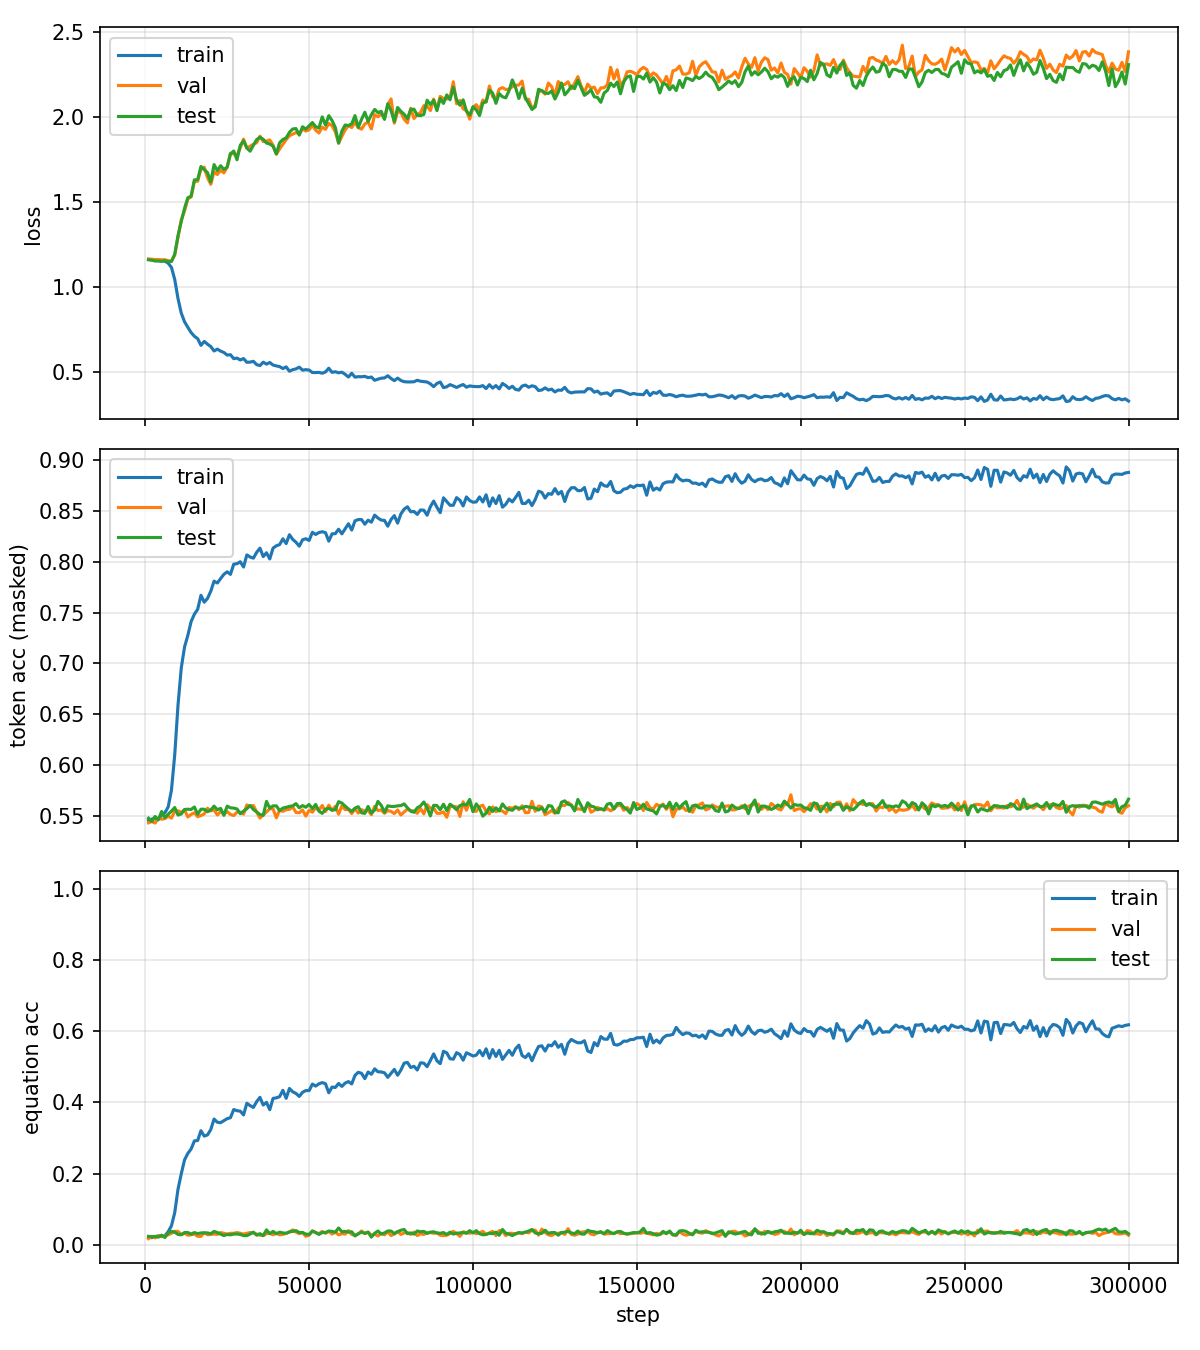
\includegraphics[width=\linewidth]{part_1/1.3/plots/part1_3_div_p97_training_curves.png}
  \caption{Training / validation / test curves for the division mod $97$ experiment (\texttt{part1\_3\_div\_p97}).}
  \label{fig:div97}
\end{figure}

\subsection{Numbers at the last logged step}

At step $300000$ (last row of \texttt{metrics.csv}), the CSV reports roughly:
\begin{itemize}[nosep]
  \item Train loss $\approx 0.331$, train token acc $\approx 0.888$.
  \item Val loss $\approx 2.38$, val token acc $\approx 0.560$.
  \item Test loss $\approx 2.31$, test token acc $\approx 0.566$.
  \item Train equation acc $\approx 0.618$; val/test equation acc stayed low on the last rows (this is consistent with the grokking story where memorization on train can run ahead of generalization on full equations).
\end{itemize}
We are not over-interpreting these here---the figure is the main takeaway for us until we write up discussion elsewhere.

\subsection{How to run inference}

From \path{deliverables/part_1/1.3/code/}, the README suggests either free-form generation or \texttt{predict\_answer} on integers. Example:
\begin{verbatim}
python inference.py --checkpoint_dir ../checkpoints/part1_3_div_p97 \
    --prompt "3 / 5 = "
\end{verbatim}

\section{What is still open}

\begin{itemize}
  \item \textbf{\S1.2:} We have smoke plots and multi-restart curves under \texttt{part\_1/1.2/plots/}, and intermediate checkpoints under \texttt{part\_1/1.2/checkpoints/}, but we still need to drop in the true final \texttt{ckpt\_100000.pt} when the long run finishes.
  \item \textbf{\S1.4:} Ablation configs exist; we still need to train, save final \texttt{ckpt\_300000.pt} for each setting, and copy the bundles into this deliverables tree.
  \item \textbf{Part~2 / Part~3:} Notebook work and the written essay are tracked separately from this summary.
\end{itemize}

\section*{Closing}

If someone only reads one thing: Part~0, \S1.1, and \S1.3 are in good shape in \texttt{deliverables/}; the rest is either partial or lives outside this folder. We will update this \texttt{.tex} file when \S1.2 and \S1.4 catch up.

\end{document}
